 % Преамбула
\documentclass[12pt, oneside, dvipsnames]{extarticle}


%вставка изображений и картинок всяких

\usepackage{graphicx}
\newcommand{\incfig}[1]{%
    \def\svgscale{1.5}
    \import{./figures/}{#1.pdf_tex}
}
\graphicspath{{pictures/}}
\DeclareGraphicsExtensions{.pdf,.png,.jpg, .jpeg, .tex}

\usepackage{booktabs} % для таблиц
\usepackage{enumitem} % для списков


% Шрифты

\usepackage[english,russian]{babel}
\usepackage[T1]{fontenc}
\usepackage{libertine}


\usepackage{titling} % для \maketitle
\usepackage{textcomp}% специальные символы в тексте

\usepackage{mathtext}
\usepackage{amsmath,amsfonts,amssymb,amsthm,mathtools} % математика
\usepackage{icomma} % умная запятая
\usepackage{import} %  импортирование


\usepackage{pdfpages} % мультри-пдф страницы
\usepackage{transparent} % что-то про цвета


\usepackage{caption} % комментарии к figure
\usepackage{epigraph} % эпиграфы

\usepackage{comment} % удобные комментарии
\usepackage{xfrac} % дроби
\usepackage{moresize} % все размеры шрифтов
\usepackage{dsfont} % mathbb для всего


% Окружения для математики:

\newtheorem{statement}{Предложение}
\newtheorem{corollary}{Следствие}
\newtheorem{theorem}{Теорема}
\theoremstyle{definition}
\newtheorem{definition}{Определение}


\newtheorem{example}{Пример}
\newtheorem{observation}{Наблюдение}
\newtheorem{homework}{Домашнее задание}
\newtheorem{antiexample}{Антиример}
\newtheorem{lemma}{Лемма}
\theoremstyle{remark}
\newtheorem*{remark}{Замечание}
\newtheorem*{exercise}{Упражнение}

% Настройки счетчиков:

%\numberwithin{equation}{section} % Number equations within sections (i.e. 1.1, 1.2, 2.1, 2.2 instead of 1, 2, 3, 4)
%\numberwithin{figure}{section} % Number figures within sections (i.e. 1.1, 1.2, 2.1, 2.2 instead of 1, 2, 3, 4)
%\numberwithin{table}{section} % Number tables within sections (i.e. 1.1, 1.2, 2.1, 2.2 instead of 1, 2, 3, 4)

% Геометрия файла:

\usepackage{geometry}

\setlist{noitemsep} % No spacing between list items

\geometry{left=1.5cm,right=1.5cm,top=2.5cm,bottom=2cm, a4paper}

% Счётчики разделов:


%\sectionfont{\vspace{6pt}\centering\normalfont\scshape} % \section{} styling
%\subsectionfont{\normalfont\bfseries} % \subsection{} styling
%\subsubsectionfont{\normalfont\itshape} % \subsubsection{} styling
%\paragraphfont{\normalfont\scshape} % \paragraph{} styling

\newcommand{\RNumb}[1]{\uppercase\expandafter{\romannumeral #1\relax}}

\renewcommand\thesection{\arabic{section}.}
\renewcommand\thesubsection{\thesection\arabic{subsection}}
\renewcommand\thesubsubsection{\RNumb{\arabic{subsubsection}}}
\renewcommand{\bf}{\textbf}

% Колонтитулы

%\usepackage{fancyhdr}
%\pagestyle{fancy}
%\fancyhf{} % clear all fields
%\fancyhead[L]{\rightmark}
%\fancyhead[R]{\thepage}

\renewcommand{\sectionmark}[1]{%
  \markright{\thesection\ #1}}%
\setlength{\headheight}{17.0pt}
\addtolength{\topmargin}{-2.49998pt}



% Операторы:

\DeclareMathOperator{\ord}{ord}
\DeclareMathOperator{\ld}{ld}
\DeclareMathOperator{\id}{id}
\DeclareMathOperator{\exi}{exi}
\DeclareMathOperator{\osc}{osc}
\DeclareMathOperator{\num}{num}
\DeclareMathOperator{\Char}{char}
\DeclareMathOperator{\card}{Card}
\DeclareMathOperator{\sk}{sk}
\DeclareMathOperator{\den}{den}
\DeclareMathOperator{\essup}{essup}
\DeclareMathOperator{\ran}{ran}
\DeclareMathOperator{\rank}{rank}
\DeclareMathOperator{\dom}{dom}
\DeclareMathOperator{\diam}{diam}
\DeclareMathOperator{\dist}{dist}
\DeclareMathOperator{\disc}{disc}
\DeclareMathOperator{\rad}{rad}
\DeclareMathOperator{\supp}{supp}

\DeclareMathOperator{\sign}{sign}
\DeclareMathOperator{\Int}{Int}
\DeclareMathOperator{\RelInt}{RelInt}
\DeclareMathOperator{\Cl}{Cl}
\DeclareMathOperator{\Class}{\mathcal{C}\mathbf{\ell}}
\DeclareMathOperator{\CW}{CW}
\DeclareMathOperator{\Ideals}{Ideals}
\DeclareMathOperator{\pr}{pr}
\DeclareMathOperator{\ind}{ind}
\DeclareMathOperator{\Af}{Aff}
\DeclareMathOperator{\Aut}{Aut}
\renewcommand{\Im}{\mathop{\mathrm{Im}}\nolimits}
\DeclareMathOperator{\Conv}{conv}
\DeclareMathOperator{\Fr}{Fr}
\DeclareMathOperator{\Tr}{Tr}
\DeclareMathOperator{\Nm}{\mathrm{N}}
\DeclareMathOperator{\Span}{span}
\DeclareMathOperator{\Map}{Map}
\DeclareMathOperator{\Hom}{Hom}
\DeclareMathOperator{\Ker}{Ker}
\DeclareMathOperator{\Ext}{Ext}
\DeclareMathOperator{\Div}{Div}
\DeclareMathOperator{\Stab}{Stab}
\DeclareMathOperator{\Fix}{Fix}
\DeclareMathOperator{\Orb}{Orb}
\DeclareMathOperator{\NRad}{NRad}
\DeclareMathOperator{\Coker}{Coker}
\DeclareMathOperator{\Gal}{Gal}
\DeclareMathOperator{\Specm}{Specm}
\DeclareMathOperator{\Spec}{Spec}
\DeclareMathOperator{\Ht}{ht}
\DeclareMathOperator{\End}{End}
\DeclareMathOperator{\Rad}{Rad}
\DeclareMathOperator{\Ann}{Ann}
\DeclareMathOperator{\Vol}{Vol}
\DeclareMathOperator{\res}{res}
\DeclareMathOperator{\Gr}{Gr}
\DeclareMathOperator{\Bl}{Bl}
\DeclareMathOperator{\mult}{mult}
\DeclareMathOperator{\cont}{cont}
\DeclareMathOperator{\area}{area}

\renewcommand{\Re}{\mathop{\mathrm{Re}}\nolimits}
\DeclarePairedDelimiter\lr{(}{)}
\DeclareRobustCommand{\divby}{%
     \mathrel{\text{\vbox{\baselineskip.65ex\lineskiplimit0pt\hbox{.}\hbox{.}\hbox{.}}}}%
}
\newcommand{\eqdef}{\stackrel{\mathrm{def}}{=}}
\DeclareRobustCommand{\notdivby}{%
     \!\!\not\;\divby%
}
\newcommand{\lei}{\trianglelefteq}

%%%% гиперссылки
\usepackage{xcolor} % цвета
\usepackage[unicode, pdftex]{hyperref}
\hypersetup{%
  colorlinks=false,
  linkbordercolor=cyan
}

% Буковы

\newcommand{\N}{\mathbb{N}}			 		
\newcommand{\Z}{\mathbb{Z}}			
\newcommand{\Q}{\mathbb{Q}}		
\newcommand{\R}{\mathbb{R}}	
\let\oldC\C
\renewcommand{\C}{\mathbb{C}} 				
\newcommand{\F}{\mathbb{F}}	
 
\let\oldAA\AA
\renewcommand{\AA}{\mathbb{A}}				
\newcommand{\DD}{\mathbb{D}}  						
\newcommand{\EE}{\mathbb{E}} 			
\newcommand{\HH}{\mathbb{H}}					
\newcommand{\KK}{\mathbb{K}} 					
\newcommand{\OO}{\mathbb{O}} 		
\newcommand{\PP}{\mathbb{P}}			
\let\oldSS\SS		
\renewcommand{\SS}{\mathbb{S}}						
\newcommand{\TT}{\mathbb{T}} 			

\newcommand{\cA}{\mathcal{A}}
\newcommand{\cB}{\mathcal{B}}
\newcommand{\cC}{\mathcal{C}}
\newcommand{\cD}{\mathcal{D}}
\newcommand{\cE}{\mathcal{E}}
\newcommand{\cF}{\mathcal{F}}
\newcommand{\cG}{\mathcal{G}}
\newcommand{\cH}{\mathcal{H}}
\newcommand{\cI}{\mathcal{I}}
\newcommand{\cJ}{\mathcal{J}}
\newcommand{\cK}{\mathcal{K}}
\newcommand{\cL}{\mathcal{L}}
\newcommand{\cM}{\mathcal{M}}
\newcommand{\cN}{\mathcal{N}}
\newcommand{\cO}{\mathcal{O}}
\newcommand{\cQ}{\mathcal{Q}}
\newcommand{\cP}{\mathcal{P}}
\newcommand{\cR}{\mathcal{R}}
\newcommand{\cS}{\mathcal{S}}
\newcommand{\cT}{\mathcal{T}}
\newcommand{\cU}{\mathcal{U}}
\newcommand{\cV}{\mathcal{V}}
\newcommand{\cW}{\mathcal{W}}
\newcommand{\cX}{\mathcal{X}}
\newcommand{\cY}{\mathcal{Y}}
\newcommand{\cZ}{\mathcal{Z}}
			
\newcommand{\rD}{\mathrm{D}}
\newcommand{\rK}{\mathrm{K}}			
\newcommand{\rP}{\mathrm{P}}
\newcommand{\rT}{\mathrm{T}}			

\newcommand{\fA}{\mathfrak{A}}
\newcommand{\fQ}{\mathfrak{Q}}
\newcommand{\fB}{\mathfrak{B}}
\newcommand{\fT}{\mathfrak{T}}
\newcommand{\fK}{\mathfrak{K}}
\newcommand{\fM}{\mathfrak{M}}
\newcommand{\fL}{\mathfrak{L}}
\newcommand{\fR}{\mathfrak{R}}
\newcommand{\fP}{\mathfrak{P}}
\newcommand{\fC}{\mathfrak{C}}
\newcommand{\fX}{\mathfrak{X}}
\newcommand{\fS}{\mathfrak{S}}
\newcommand{\fH}{\mathfrak{H}}

\newcommand{\fm}{\mathfrak{m}}
\newcommand{\fb}{\mathfrak{b}}
\newcommand{\ff}{\mathfrak{f}}
\newcommand{\fp}{\mathfrak{p}}
\newcommand{\fq}{\mathfrak{q}}
\newcommand{\fh}{\mathfrak{h}}
\newcommand{\fo}{\mathfrak{o}}
\newcommand{\fe}{\mathfrak{e}}
\newcommand{\ft}{\mathfrak{t}}
\newcommand{\fr}{\mathfrak{r}}
\newcommand{\fg}{\mathfrak{g}}
\newcommand{\fl}{\mathfrak{l}}
\newcommand{\fa}{\mathfrak{a}}
\newcommand{\fd}{\mathfrak{d}}
\newcommand{\qAff}{\mathsf{qAff}}
\newcommand{\Aff}{\mathsf{Aff}}
\newcommand{\Alg}{\mathsf{Alg}}
\newcommand{\Set}{\mathsf{Set}}
\newcommand{\Mod}{\mathsf{Mod}}
\usepackage{esint}
\renewcommand{\v}{\upsilon}
\newcommand{\vp}{\v_{p}}

% Tikz и графика:


\usepackage{pgfplots}
\usepackage{tikz}
\usetikzlibrary{3d,perspective}
\usetikzlibrary{animations}
\usetikzlibrary{cd}
\usepackage{mathtools}
\pgfplotsset{width=6cm,compat=newest}

\newcommand{\RNum}[1]{\uppercase\expandafter{\romannumeral #1\relax}}

\usepackage{amssymb} 
\def\acts{\curvearrowright}



\usepackage{cleveref}
\usepackage[
backend=biber,
style=alphabetic,
sorting=ynt
]{biblatex}
\addbibresource{mybib.bib}

\begin{document}
	
	\begin{center}
	{ \Huge \bf{Древесные симметрии} }

	\section*{Проекты}
	\end{center}

	\tableofcontents

	\begin{center}
		\subsection*{Стабилизация лучей и параболические подгруппы}
		\addcontentsline{toc}{subsection}{\protect\numberline{}Стабилизация лучей и параболические подгруппы}%
	\end{center}

	\begin{definition} 
		Пусть $X^*$~--- регулярное корневое дерево, $e$ луч, а $G \le \Aut(X^*)$~--- произвольная подгруппа. Тогда \emph{ассоциированная с $G$ параболическая подгруппа  $P_{e}$}~--- это $\Stab_{G}(e)$. 
	\end{definition}

	Иными словами, параболические подгруппы~--- это подгруппы, стабилизирующие лучи в $X^*$ (или же, точки $\partial X$). 

	Базовые (и несложные) факты про параболические подгруппы изложены в~\cite[стр. 8-9]{bartholdi2001parabolic} (всего несколько страничек).


	Введём несколько важных для нас групп, действующих на корневых деревьях. 

	\begin{definition} 
		Пусть $p$~--- простое число, $T_{p}$~--- $p$-регулярное корневое дерево. Группой \bf{$p$-базилики $\fB_{p}$} называется подгруппа в $\Aut(T_{p})$, порожденная элементами 
		 $$ a = (1,1, \ldots ,1,b), \quad b = (1,1, \ldots ,1,a)\sigma, \quad \text{ где } \sigma = (1 2  3 \ldots p) \in S_{p} $$

		 Прочитать подробнее про неё можно в~\cite{didomenico2021pbasilica}.
	\end{definition}

	\begin{definition} 
		\bf{$\mathbf{GGS}$-группой (или же группой Григорчука-Гупты-Сидки)} называется, подгруппа $\langle a, \sigma \rangle$ в $\Aut(T_{p})$, порожденная циклической перестановкой $\sigma = (123 \ldots p)$  и элементом 
		$$ a = (\sigma^{e_1},\sigma^{e_2},...,\sigma^{e_{p-1}},a), $$
		где $e_i \in \F_{p} = \Z/p\Z$.
	\end{definition}

	Подробнее о $\mathbf{GGS}$-группах и связанных с ними результатах про рост вы можете прочитать в работе~\cite{didomenico2022ggsgroups}. 

	\begin{definition} 
		Группа \bf{Гупты-Фабриковского} определяется следующим образом. Рассмотрим $A = C_{p} = \langle a \vert a^p = 1 \rangle $  и $p$-регулярное корневое дерево $A^* = T_p$.  Заметим, что тогда $a$ мы можем отождествить с циклической перестановкой $\sigma = (1 2 p)$, действующей на первом уровне. Определим автоморфизм $t \in \Aut(A^*) \cong \Aut(A^*) \wr S_{p} $, как $t = (a, 1, t)$. Заметим, что элементы $a$ и $t$ имеют порядок $p$. Группа $\mathbf{\Gamma} = \langle a, t \rangle \le \Aut(A^*)$ и будет называться группой \bf{Гупты-Фабриковского} порядка $p$. 
	\end{definition}

	Подробнее об этой группе и связанных с ней результатах про рост вы можете прочитать в работе Л. Бартольди~\cite{Bartholdi_2009}. 

	Кроме них, все мы помним про \bf{группу Григорчука $\mathbf{G}$}. 

	Все эти группы отличаются красотой и незаурядностью в их действии на деревьях и в связи с этим представляют видимый научный интерес. Про них предлагаются такие задачи: 

	\begin{enumerate}
		\item Для каждой группы посчитать параболические группы каких-то бесконечных лучей и изучить факторы по ним, возможно их рост.

		\item Правда ли, что елсли отфакторизовать группу 3-Базилики $\fB_{3}$ по параболической подгруппе $P_{e} = \Stab_{fB_{3}}(e)$, стабилизирующий некоторый луч в 3-регулярном дереве, группа $3$-базилики превратится в группу 2-базилики. И, если нет, то каков результат факторизации? 
	\end{enumerate}




	\begin{center}
		\subsection*{О модификации групп}
		\addcontentsline{toc}{subsection}{\protect\numberline{}О модификации групп}%
	\end{center}

	Понятие регулярного корневого дерева $T_{d}$ можно естественно обобщить следующим образом: 

	\begin{definition} 
		Пусть $\overline{m} = \{ m_n \}, m_n \ge 2$~--- последовательность натуральных чисел. \emph{Сферически однородным корневым деревом} $T_{\overline{m}}$ мы будем называть корневое дерево, имеюще такой вид: 	
		\begin{itemize}
			\item У него есть корень $\varnothing$, а также 
			\item $m_1$ вершин первого уровня, $m_1 m_2$ вершин второго уровня, \ldots, $m_1 m_2 \ldots m_n$ вершин $n$-го уровня ($n \in \N$).
			\item Каждая вершина уровня $n$ имеет $m_{n + 1}$ детей, расположенных на следующем уровне.
		\end{itemize}
	\end{definition}	

	\begin{figure}[tbph]
		\centering
		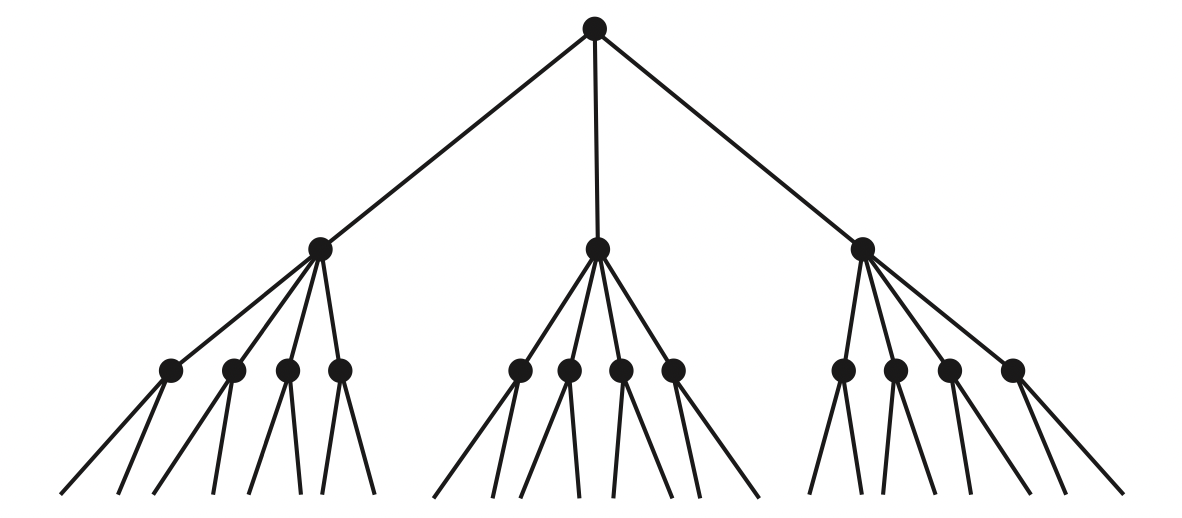
\includegraphics[scale = 0.5]{pictures/pic_3.png}
		\caption{Сферически однородное корневое дерево}
		\label{fig:pic_3.png}
	\end{figure}

	Более подробную информацию о них можно прочитать в работе Р.И. Григорчука~\cite[стр. 80 и далее]{Grig_Sperical}. 

	Так как эти деревья естественно обобщают $T_{d}$, возникает вопрос о нетривиальных вложениях $ G  \hookrightarrow \Aut(T_{\overline{m}})$ для различных подгрупп $G \le \Aut(T_{d})$. В связи с этим предлагаются следующие задачи: 

	\begin{enumerate}
		\item Предлагается изучить способы вложения групп $p$-базилики $\fB_{p}$, Гупты-Фабриковского, $\mathbf{GGS}$-групп в $\Aut(T_{\overline{m}})$. Возможно, вычислить количество вложений. 

		\item Попытаться  вложиьб группу 2-Базилики и группу Григорчука $\mathbf{G}$ в дерево с последовательностью слоев $(23)^\infty$.
	\end{enumerate}


	\begin{center}
		\subsection*{Геометрический проект}
		\addcontentsline{toc}{subsection}{\protect\numberline{}Геометрический проект}%
	\end{center}

	Существует понятие \bf{константы гиперболичности пространства}. Это число $\delta$, ассоциированное с ним и отвечающее тому, насколько его геометрия похожа на гиперболическую. 

	К сожалению этот инвариант работает так, что если $\delta < \infty$, то пространство "очень" гиперболическое, а если $\delta = \infty$, то всё, что мы знаем это то, что оно другое. То есть разделение очень дискретное, а хотелось бы критерия в духе "чем больше число тем более гиперболическое пространство".

	Чтобы избавиться от такой большой критичности, можно по каждому пространству $M$ определить функцию $\delta_M$, которая будет исполнять ровно такую роль. Это очень \bf{новый} инвариант и про него непонятно вообще ничего. 

	\noindent\bf{Предлагается две задачи:}
	\begin{enumerate}
		\item Построить примеры метрических пространств, у которых эта функция будет устроена определенным образом (заранее заданным).
		\item Вычислить эту функцию для конкретного пространства --- графа определенного вида. 
	\end{enumerate}

	\emph{Никаких конкретных пререквезитов не предполагается.}

	\printbibliography

\end{document}